\documentclass[10pt, onecolumn, draftclsnofoot, letterpaper, compsoc]{IEEEtran}

\usepackage{cite}
\usepackage{float}
\usepackage{hyperref}
%\usepackage{enumitem}
\usepackage{graphicx}

% Macro for the signatures
\newcommand*{\SignatureAndDate}[1]{%
    \par\noindent\makebox[2.5in]{\hrulefill} \hfill\makebox[2.0in]{\hrulefill}%
    \par\noindent\makebox[2.5in][l]{#1}      \hfill\makebox[2.0in][l]{Date}%
}

\renewcommand*\contentsname{Table of Contents} % Rename ToC

\newcommand{\myindent}{\hspace{\oldparindent}}

% Temp title and author
\title{Design Document}
\author{Totality AweSun \\
		Bret~Lorimore, Jacob~Fenger, George~Harder \\
		\textit{\today \\
		CS 461 - Fall 2016}}

\begin{document}

\maketitle

\begin{abstract}

This document describes in detail the design for the various components of the
North American Solar Eclipse 2017 senior capstone project. These components are
described according to the IEEE 1016-2009 standard. There are three high level
components detailed in this document, the Eclipse Image Processor, Eclipse Image
Processor Manager, and Eclipse Simulator. The sections of this document are broken
into subsections corresponding to these components as applicable.

\end{abstract}

\vspace{10mm}
\noindent \SignatureAndDate{David Konerding, Project Sponsor}
\vspace{8mm}
\noindent \SignatureAndDate{Bret Lorimore}
\vspace{8mm}
\noindent \SignatureAndDate{George Harder}
\vspace{8mm}
\noindent \SignatureAndDate{Jacob Fenger}

\newpage

\tableofcontents

\newpage

%% Section 1
\section{Design Stakeholders and Their Concerns}

The primary stakeholder in this project is David Konerding of Google.
He is one of the managers of the Eclipse Megamovie project that is sponsoring
this Senior Capstone project. David Konerding's concerns are listed below.

\subsection{Image Processor}

\subsubsection{}

The image process needs to take in an image, identify if the image has a total
solar eclipse, and if it does further process it so that it can be stitched into
a timelapse movie by Eclipse Megamovie engineers. \\

\subsubsection{}

The mean processing time for an image must be one second. \\

\subsubsection{}

Images must be processed in no longer than five seconds.\\

\subsubsection{}

Images must be filtered so that the processed images are only images of the
eclipse at totality.\\

\subsubsection{}

Only high quality images, defined as having a 50 pixel solar disk size and
padding around the disk of 100 pixels, should be accepted by the image
processor.\\

\subsubsection{}

Once images have been filtered, they need to have metadata attached in a way
that allows easy stitching of eclipse images. \\

\subsubsection{}

The image processor needs to be able to be called by the image processor manager
with appropriate input data. \\

\subsubsection{}

Image processor needs to be able to use GPS EXIF information associated with
images.\\

\subsection{Image Processor Manager}

    \subsubsection{}
    Image processor manager should download images needing processing
    from Google Cloud Storage. \\

    \subsubsection{}
    Image processor manager should invoke image processor with downloaded images. \\

    \subsubsection{}
    Image processor manager should upload processed images and corresponding metadata
    - the output from the image processor - to Google Cloud Storage and Datastore, respectively. \\

    \subsubsection{}
    Image processor should download/upload images at the same time the image processor
    is processing other images. \\

    \subsubsection{}
    Image processor manager should invoke multiple image processor instances concurrently
    with different input images. The number of image processor instances launched should be
    determined by the number of cores on the host VM. \\

    \subsubsection{}
    Image processor manager instances should be able to run alongside other image processor
    manager instances running on (potentially) different machines. These discrete instances should
    not attempt to process the same images. \\

\subsection{Eclipse Simulator}
    \subsubsection{}
    The solar eclipse must be accurately simulated based on
    user entered location information. \\

    \subsubsection{}
    Users will be able to adjust simulator time via a
    draggable slider or clickable buttons. \\

    \subsubsection{}
    Simulator will only support locations within continental
    United States. \\

    \subsubsection{}
    The simulator must load in less than 500ms given a 1-10
    Mbps internet connection. \\


%% Section 2
\section{Design Viewpoints}

\subsection{Image Processor}

\subsubsection{Speed and Performance}

\textbf{Concerns:} 1.1.2, 1.1.3 \\
\textbf{Elements:} 4.1.1, 4.1.2, 4.1.3, 4.1.4\\
\textbf{Analytical Methods:} The primary criteria and methods in constructing
this view is whether or not we are achieving the desired average speeds on our
golden data set. \\
\textbf{Viewpoint Source:} George Harder \\

\subsubsection{Accuracy}

\textbf{Concerns:} 1.1.1, 1.1.4, 1.1.5, 1.1.8 \\
\textbf{Elements:} 4.1.1, 4.1.2, 4.1.5, 4.1.6 4.1.9, 4.1.10\\
\textbf{Analytical Methods:}  In constructing the corresponding view, we will be
evaluating it based on whether or not the image processor is correctly
identifying eclipses with at least 90\% accuracy on our golden data set.\\
\textbf{Viewpoint Source:} George Harder \\

\subsubsection{Input and Output}

\textbf{Concerns:} 1.1.6, 1.1.7 \\
\textbf{Elements:} 4.1.2, 4.1.4, 4.1.7, 4.1.8, 4.1.9\\
\textbf{Analytical Methods:} This view will be evaluating whether or not the
input and output of the image process meet the specifications defined in the
design document. \\
\textbf{Viewpoint Source:} George Harder\\

\subsection{Image Processor Manager}

    \subsubsection{Intra-instance Concurrency}
    \textbf{Concerns:} 1.2.4, 1.2.5 \\
    \textbf{Elements:} 4.2.1, 4.2.2, 4.2.3, 4.2.4, 4.2.5, 4.2.6, 4.2.7 \\
    \textbf{Analytical Methods:} Overall VM CPU utilization, overall VM network interface utilization.
    Both these values should be maximized as much as possible. \\
    \textbf{Viewpoint Source:} Bret Lorimore \\

    \subsubsection{Inter-instance Concurrency and Synchronization}
    \textbf{Concerns:} 1.2.1, 1.2.3, 1.2.6 \\
    \textbf{Elements:} 4.2.1 \\
    \textbf{Analytical Methods:} No image should be successfully processed by multiple image processor
    instances, whether or not these run on the same VM or are managed by the same image processor manager. \\
    \textbf{Viewpoint Source:} Bret Lorimore \\

    \subsubsection{Invocation}
    \textbf{Concerns:} 1.2.2 \\
    \textbf{Elements:} 4.2.6 \\
    \textbf{Analytical Methods:} Multiple image processor processes should be able to be easily launched
    concurrently with different input data. \\
    \textbf{Viewpoint Source:} Bret Lorimore \\

\subsection{Eclipse Simulator}
  \subsubsection{Interface}
  \textbf{Concerns:} 1.3.1, 1.3.2 \\
  \textbf{Elements:} 4.3.1, 4.3.2, 4.3.4, 4.3.7 \\
  \textbf{Analytical Methods:} Interface should be appealing
  to the user as well as being responsive and fast. \\
  \textbf{Viewpoint source:} Jacob Fenger \\

  \subsubsection{Loading Performance}
  \textbf{Concerns:} 1.3.4\\
  \textbf{Elements:} 4.3.3, 4.3.4, 4.3.5, 4.3.6, 4.3.7 \\
  \textbf{Analytical Methods:} The initial loading time
  of the simulator should be fast. Additionally, the
  interactions that the user has with the simulator should
  be responsive and should not show any significant slow
  downs. \\
  \textbf{Viewpoint source:} Jacob Fenger \\

  \subsubsection{Simulation Accuracy}
  \textbf{Concerns:} 1.3.1, 1.3.3 \\
  \textbf{Elements:} 4.3.3, 4.3.5 \\
  \textbf{Analytical Methods:} In the simulator, the Sun and
  Moon display should reflect scientific accuracy when it
  comes to relative position and sizes. Additionally, the
  view of the Sun and Moon above the horizon shall be
  accurate.\\
  \textbf{Viewpoint source:} Jacob Fenger \\


%% Section 3
\section{Design Views}

\subsection{Image Processor}

\subsubsection{Speed and Performance [Governed by Viewpoint 2.1.1]}

The Eclipse Megamovie project expects to receive photographs on the order of
hundreds of thousands from the numerous citizen photographers registered with
the project. This being the case, it is of utmost importance that the image
processor we are building for the project can process images in a timely manner.
This is not only important to being able to build a movie from the images soon
after the eclipse, but also because it prevents storage spaces on either end of
the image processing pipeline from becoming clogged. \\

In order to achieve these design goals, we are designing a system that uses the
OpenCV C++ library.  This API provides us with high performing library methods,
like Hough transforms, image crops, and image rotations that are necessary to
the image processor's core functionality. In addition to the use of this
language and library, we are also designing this system to be single threaded
but to also interface with a manager that runs multiple instances of the image
processor concurrently. This fact allows us to design the image process to
process a single image quickly and accurately and leaves management of the
application to a different art of the system.\\

\subsubsection{Accuracy [Governed by Viewpoint 2.1.2]}

From a high level, the most fundamental concern in the design of the image
processor is that it can accurately identify an eclipse image. The other
concerns associated with the design of the image processor are near meaningless
if the application is not consistently identifying images that contain total
eclipse.\\

To address this concern, and the related concerns around accepting only high
quality images and determining the relative temporal and spatial positioning of
images, we are designing this application with accuracy as a primary goal. The
meet this goal, the system will build upon an existing eclipse identification
algorithm. This algorithm, with improvements we add ourselves, will be the basis
for the parts of the system that we design to meet the accuracy requirements of
the image processor.\\

\subsubsection{Input and Output [Governed by Viewpoint 2.1.3]}

The image processor is one component in a much larger system. For the system to
function the image processor needs to interface with the other components in a
well defined and seamless manner. In addition to speed and accuracy, we need to
design the system with a view toward optimizing the way the image processor
interacts with other components.\\

The ensure a smooth interface with the image processor manager we are designing
the image processor to accept a well defined set of command line arguments
including the path to the list of images to be processed, the path to an output
directory, and the path to prefix image file names with that points to their
location. The design of the image processor also takes into account the needs of
the engineers handling the processed images. The image processor will write
processed images and their metadata in a specific format to an output file.\\

\subsection{Image Processor Manager}

    \subsubsection{Maximal Utilization [Governed by viewpoint 2.2.1]}
    It is the goal of the image processor manager to maximize hardware utilization on the VMs on which it is
    running. This means that ideally, the VMs where the image processor manager and therefore the image
    processor are running will have an average of 100\% CPU utilization on all cores at all times.The image
    processor application will be single threaded and thus by invoking multiple instances of this application,
    the image processor manager can increase utilization on multiple CPU cores. \\

    The downloading of images to process and uploading of processed images are both very high latency
    operations. Therefore, instead of waiting for these downloads/uploads to complete with virtually zero CPU
    utilization in the meantime, the image processor manager can achieve greater average CPU utilization by
    completing these high latency tasks concurrently to processing other images. \\

    \subsubsection{Image Processing [Governed by viewpoint 2.2.2]}
    The ultimate goal of the image processor manager is to facilitate the processing of eclipse images by the
    image processor component of this project. This can be achieved by downloading images to process from the
    cloud, assembling them into a form that can be consumed by the image processor and then invoking that
    application with the downloaded images as input data. \\

    \subsubsection{Synchronization [Governed by viewpoint 2.2.3]}
    The image processor must process the images that are uploaded by users. These images are uploaded by the
    eclipsemega.movie website to Google Cloud Storage and metadata entries are also created for them in Google
    Cloud Datastore. In order for the image processor manager to invoke the image processor with these images,
    it must download them from Google Cloud. \\

    The application to stitch processed images into movies, being developed by Google, expects to find
    processed eclipse images in Google Cloud Storage with corresponding metadata in Google Cloud Datastore. In
    order to meet this expectation, the image processor manager must upload the results of running the image
    processor to Google Cloud Storage and Google Cloud Datastore when ready. \\

    To enable scalable image processing performance, it is desirable to enable many VMs to run image processor
    applications at once. In order to do this efficiently without redundancy, it is necessary to ensure that
    multiple VMs do not try to process the same images. For that reason, image processor manager instances must
    mark image files as pending processing before another instances of the image processor manager can queue
    them for processing. Without implementing this functionality, little to no performance improvements can be
    expected by deploying multiple image processor manager nodes. \\

\subsection{Eclipse Simulator}

  \subsubsection{User Interface View [Governed by Viewpoint 2.3.1 ]}
  The user interface shall utilize 2D animated depictions of
  the Sun and the Moon as they appear at a user specified
  time and location. In addition, the user interface will
  contain background imagery such as a city or hillside
  landscape. There will also be a time slider, a location
  input, and a time display for users to interact with or
  view. \\

  \subsubsection{Operating Performance View [Governed by Viewpoint 2.3.2]}
  The simulator will have low loading times to ensure fast
  performance for most users. Additionally, the simulator
  will need to respond in a timely matter when users are
  interacting with the module. \\

  \subsubsection{Eclipse Accuracy View [Governed by Viewpoint 2.3.3]}
  The simulator shall be accurate enough for any location in
  the continental United States. This accuracy includes
  accurate relative Moon and Sun sizes, positions in the
  rendered scene, and positions relative to one another. \\

%% Section 4
\section{Design Elements}

\subsection{Image Processor}

\subsubsection{OpenCV}
\textbf{Type:} Library\\
\textbf{Purpose:} OpenCV is the computer vision library we will use to process
images. This open source library can quickly crop and otherwise manipulate
images. It best suits our needs for a computer vision utility.\\

\subsubsection{C++}
\textbf{Type:} Class\\
\textbf{Purpose:} This application will be written in C++ in order to give us
better control over the speed at which the application runs and the necessary
functionality for reading and writing files. \\

\subsubsection{Image Processing Time}
\textbf{Type:} Constraint\\
\textbf{Purpose:} This element exists because our requirements specify that the
average time for an image to be processed must be less than one second.\\

\subsubsection{Serial Image Processing}
\textbf{Type:} Framework\\
\textbf{Purpose:} The image processor will process images one at a time because
the Image Processor Manager handles all parallelization.\\

\subsubsection{Hough Transform}
\textbf{Type:} Procedure\\
\textbf{Purpose:} The Hough transform is an algorithm for identifying circles
and lines in images. It will be used by the image processor to identify total
eclipse images. OpenCV has the circular Hough transform built in. \\

\subsubsection{Image Quality Error Checking}
\textbf{Type:} Constraint\\
\textbf{Purpose:} The requirements of the image processor specify that only
images with a solar disk of at least 50 pixels and 100 pixels of padding around
the sun will be accepted.\\

\subsubsection{Command Line Arguments}
\textbf{Type:} Constraint\\
\textbf{Purpose:} The image processor needs to have a well defined set of
command line arguments so that it can interface with the image processor
manager without difficulty. \\

\subsubsection{Data writer}
\textbf{Type:} System\\
\textbf{Purpose:} This component is meant to encapsulate the functionality
necessary to write the processed images and their associated metadata to an
output file.\\

\subsubsection{Image Data Structure}
\textbf{Type:} Class\\
\textbf{Purpose:} This class will encapsulate the information and methods needed
to manage the images we will be processing. It will also work closely with the
Data Writer to write images and their metadata to files.\\

\subsubsection{Solar Eclipse Image Standardisation and Sequencing (SEISS)}
\textbf{Type:} Procedure\\
\textbf{Purpose:} The SEISS algorithm is an image processing algorithm that can
identify images of eclipses, including eclipses at totality \cite{imgKrista}. We
will be basing part of the image processor off of this algorithm. \\

\subsection{Image Processor Manager}

    \subsubsection{Image List Downloader}
    \textbf{Type:} Subsystem \\
    \textbf{Purpose:} The purpose of this subsystem is to download and return a list of images from Datastore
    to be processed by the image processor application. It will use Datastore transactions to ensure that each
    image in this list is marked as pending processing before it can be retrieved by another image processor
    manager instance. The max number of image files retrieved will be determined by the number of image
    processor processes that are going to be launched. This value will be a parameter of the image list
    downloader subsystem. \\

    \subsubsection{Image Downloader}
    \textbf{Type:} Subsystem \\
    \textbf{Purpose:} The purpose of this subsystem is to download and save individual image files. It will
    accept the name of an image file to retrieve from Cloud Storage and a place to store this file, and will
    then download the file and save it to the desired location. \\

    \subsubsection{Image Download Manager}
    \textbf{Type:} System \\
    \textbf{Purpose:} The purpose of this system is to coordinate design elements 4.2.1 and 4.2.2, the
    \textit{Image List Downloader} and \textit{Image Downloader}, respectively. It will use the
    \textit{Image List Downloader} to retrieve a list of images to download and then will use the Python
    multiprocessing module to launch multiple instances of the \textit{Image Downloader} subsystem
    concurrently to download the images in the list. \\

    \subsubsection{Result Uploader}
    \textbf{Type:} Subsystem \\
    \textbf{Purpose:} The purpose of this subsystem is to upload an individual processed image to Google Cloud
    Storage and upload its metadata to Google Cloud Datastore. \\

    \subsubsection{Result Uploader Manager}
    \textbf{Type:} System \\
    \textbf{Purpose:} The purpose of this system is to coordinate element 4.2.4, the \textit{Results Uploader}.
    It will use the Python multiprocessing module to launch multiple instances of the \textit{Results Uploader}
    concurrently to upload the output of the image processor. \\

    \subsubsection{Image Processor Invoker}
    \textbf{Type:} System \\
    \textbf{Purpose:} The purpose of this system is to invoke multiple instances of the image processor
    application concurrently using the Python subprocess module. It will distribute images to process over
    multiple image processor processes to increase throughput. The number of image processor processes will be
    determined by the number of cores on the host VM. \\

    \subsubsection{Controller}
    \textbf{Type:} System \\
    \textbf{Purpose:} The purpose of this system is to coordinate the three other systems that are part of the
    image processor manager, design elements 4.2.3, 4.2.5, and 4.2.6, the \textit{Image Download Manager},
    the \textit{Result Uploader Manager}, and the \textit{Image Processor Invoker}. It will run these systems
    in parallel so that images are downloaded/uploaded at the same time that other images are being
    processed. \\


\subsection{Eclipse Simulator}

  \subsubsection{Scalar Vector Graphics (SVG)}
  \textbf{Type:} System \\
  \textbf{Purpose:} This element shall be used for the
  front-end display of the eclipse simulator.
  Two-dimensional images of the Sun and Moon will be altered
  based on how the user interacts with the module.


  \subsubsection{Cascading Style Sheets (CSS)}
  \textbf{Type:} System \\
  \textbf{Purpose:} CSS helps with the front-end display of
  the simulator by helping produce better looking output.

  \subsubsection{Ephemeris JavaScript Library}
  \textbf{Type:} Library \\
  \textbf{Purpose:} This library is used to compute eclipse
  information to be used for displaying the Sun and Moon.

  \subsubsection{View}
  \textbf{Type:} Component \\
  \textbf{Purpose:} Combined the HTML, SVG, and CSS elements
  for simulator display and interaction for the user.

  \subsubsection{Model}
  \textbf{Type:} Component \\
  \textbf{Purpose:} Backend library in JavaScript used for
  computing eclipse information which will be passed to the
  controller. This entity utilized the Ephemeris JavaScript
  library for support.

  \subsubsection{Controller}
  \textbf{Type:} Component \\
  \textbf{Purpose:}  Controls the interaction between the
  model and view. Information will be passed between these
  entities.

  \subsubsection{Model-View-Controller Architecture}
  \textbf{Type:} Relationship \\
  \textbf{Purpose:} This architecture is defined by the interactions of the model, view, and controller entities.

%% Section 5
\section{Design Overlays}

\subsection{Image Processor}

\begin{figure}[H]
    \centering
    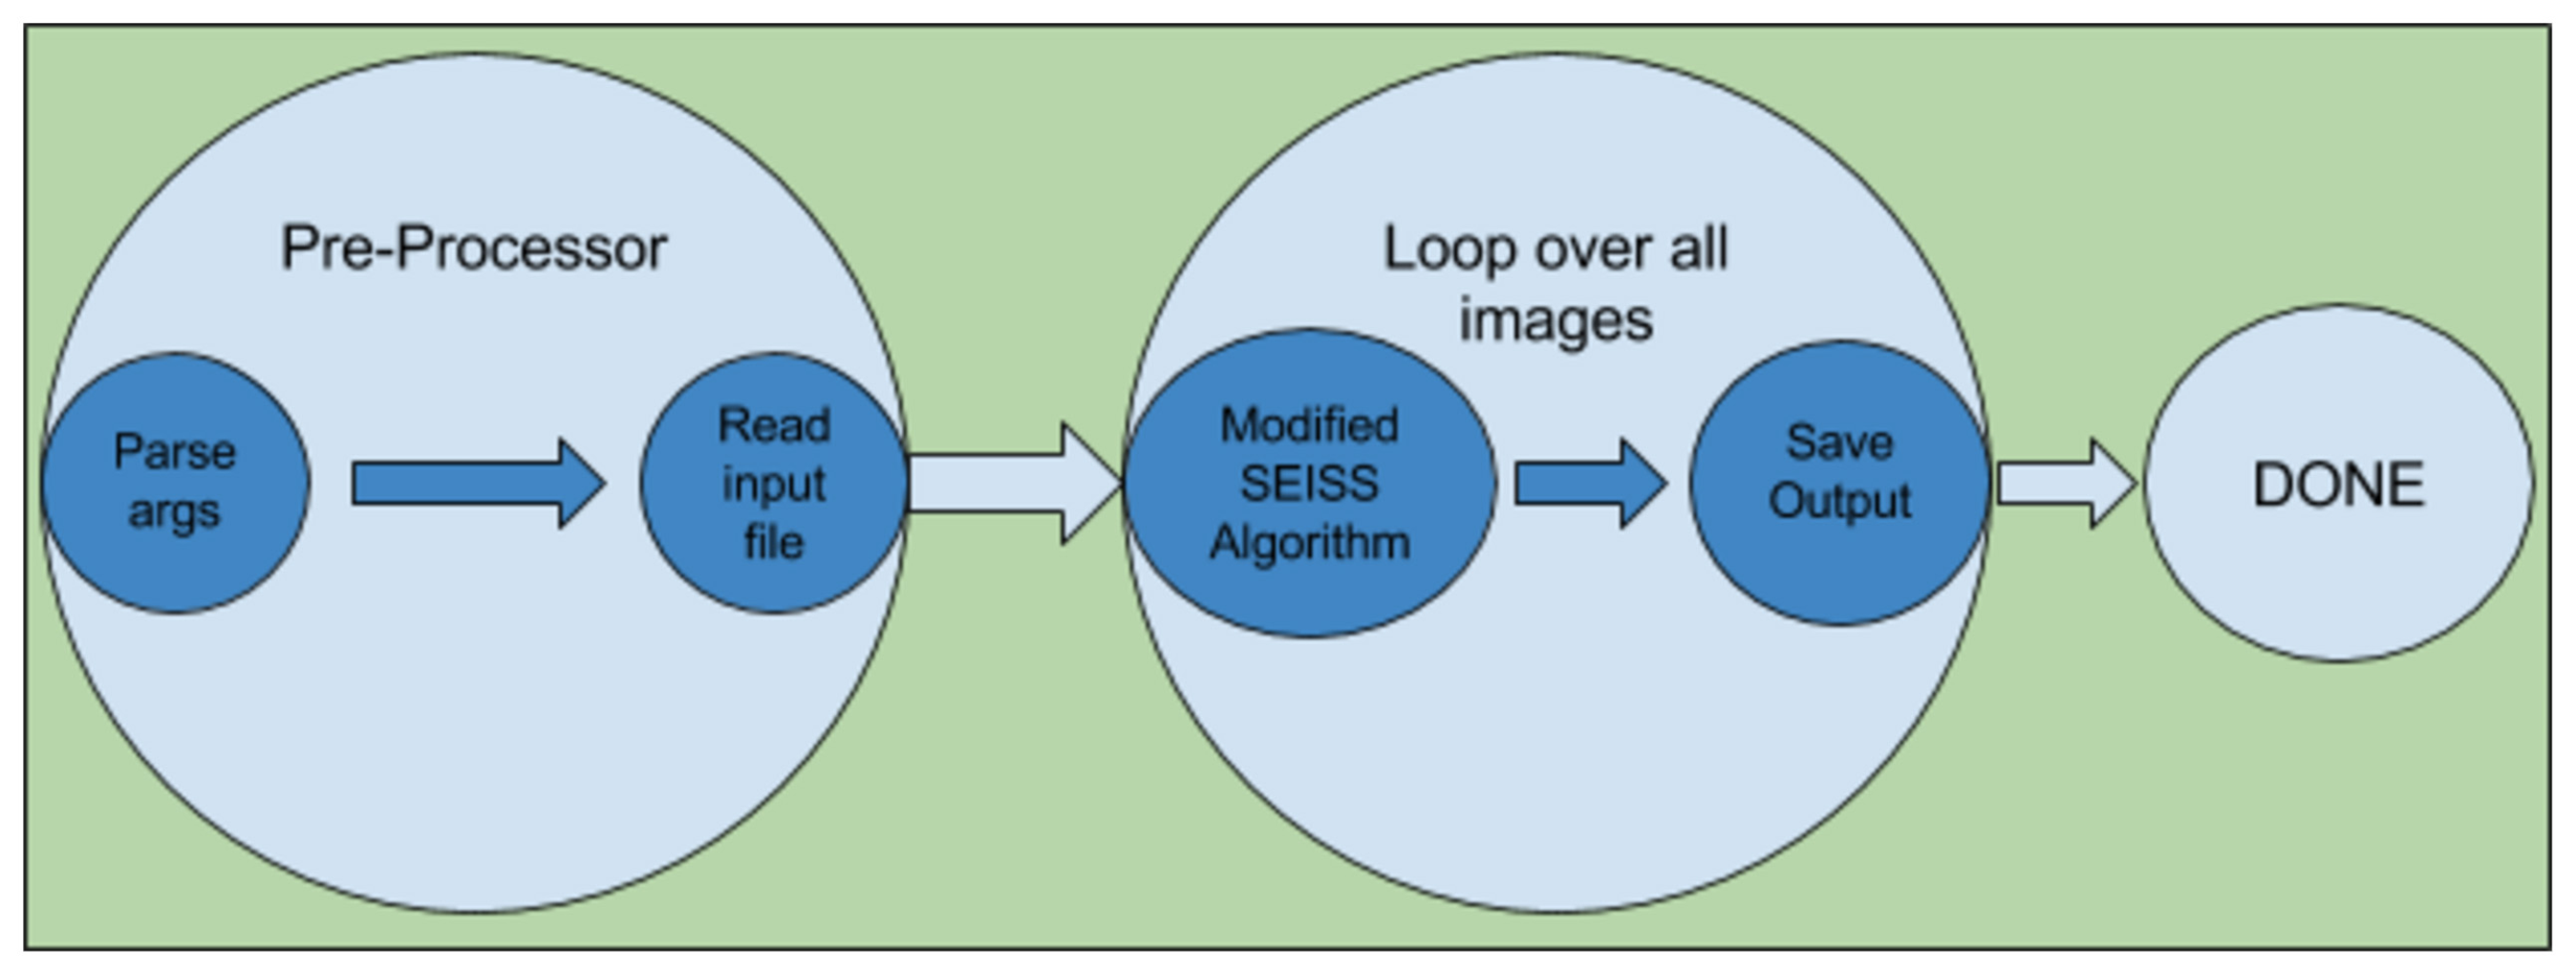
\includegraphics[width=\textwidth]{george_fig.eps}
    \caption{Image processor basic dataflow}
\end{figure}

\subsection{Image Processor Manager}

\begin{figure}[H]
    \centering
    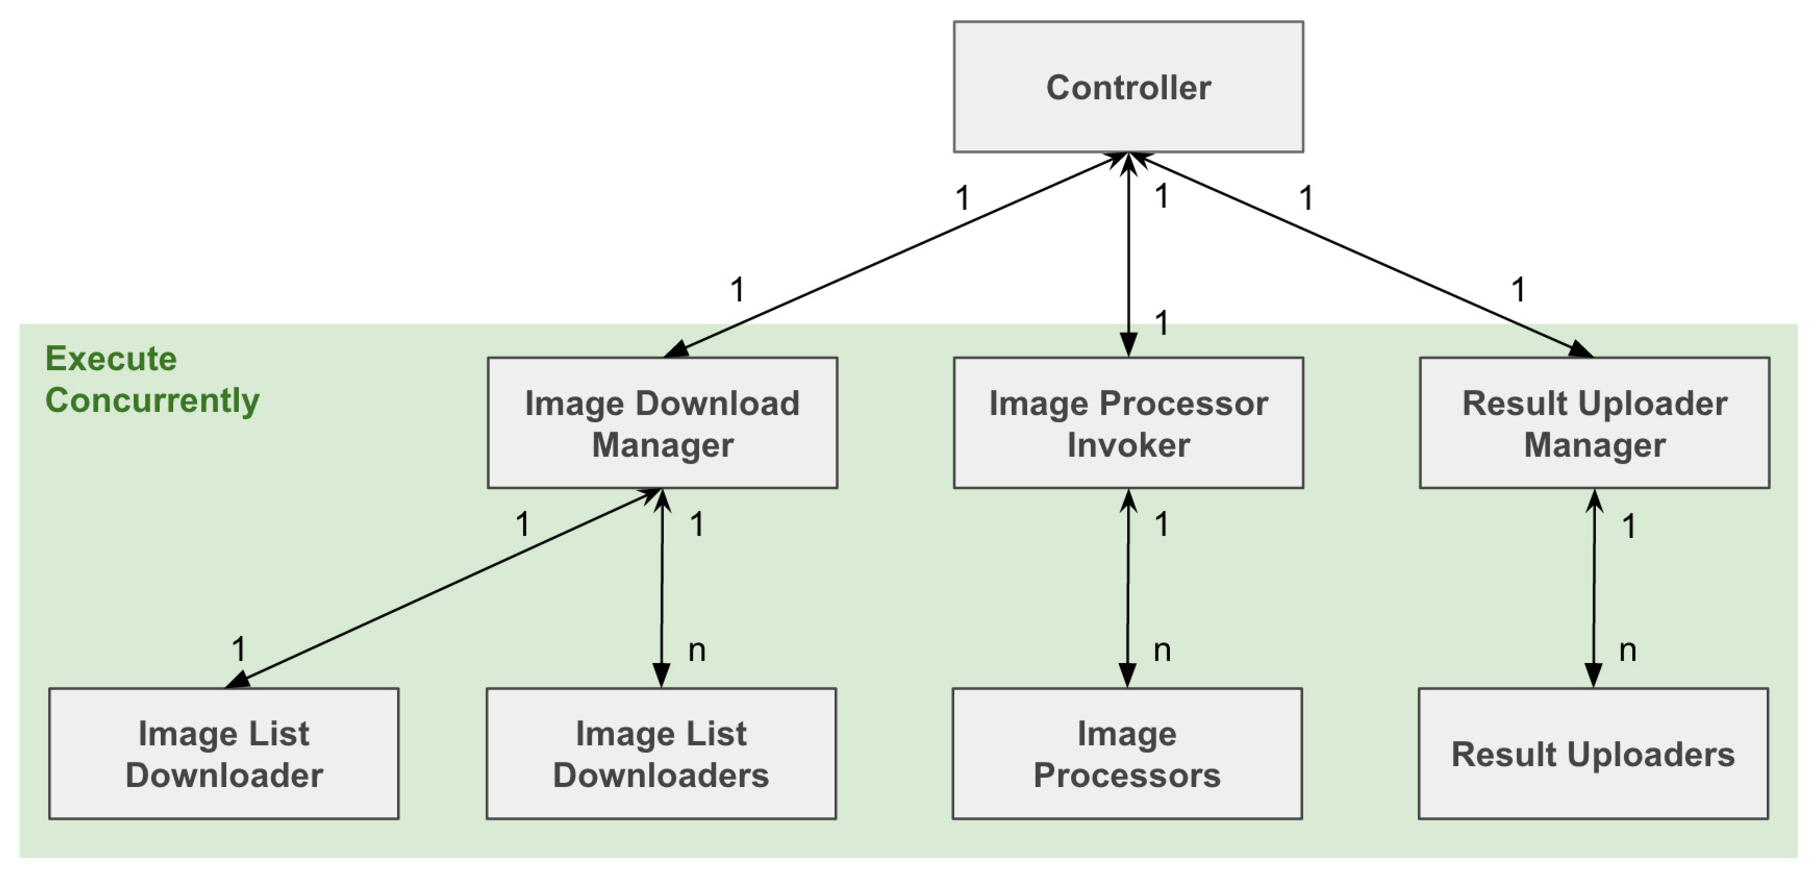
\includegraphics[width=0.75\textwidth]{bret_fig.eps}
    \caption{Image processor manager system diagram [Associated with Viewpoint 2.2.1]}
\end{figure}

\subsection{Eclipse Simulator}

\begin{figure}[H]
    \centering
    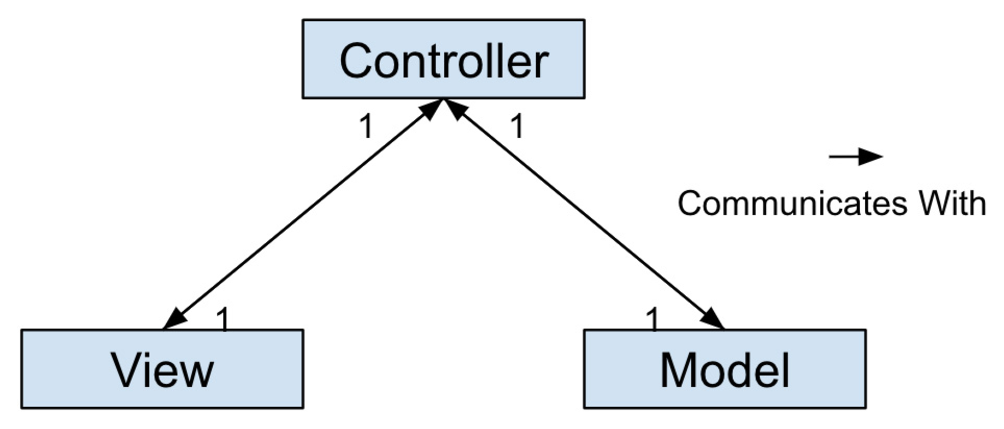
\includegraphics[width=0.5\textwidth]{jake_fig.eps}
    \caption{Eclipse simulator MVC architecture}
\end{figure}


%% Section 6
\section{Design Rationale}

\subsection{Image Processor}

The design of this system is based on needs surrounding accuracy, speed, and
ability to interface with other components in the larger system. As was detailed
in the technology review, we made certain decisions about what tools and
algorithms to use based on the specific requirements of our system. The use of
these tools has necessarily shaped the design of this application.\\

Additional information regarding design rationale can be found in the 'Purpose'
section of the design elements.

\subsection{Image Processor Manager}

    \subsubsection{High Level System Design}
    From a high level the system is designed to be highly parallel with the aim of achieving as close to
    100\% CPU utilization on all cores as possible. In order to achieve this it is necessary to ensure that
    images to process are downloaded ahead of the time they're needed, this way the latency of their download
    time is hidden by processing other images. It is also necessary to ensure that processed images do not back
    up. The design elements outlined above fit together to form a system that naturally supports a very high
    level of concurrency. Subsystems to handle individual tasks are built and then multiple instances of these
    subsystems can be launched concurrently with different parameters. These subsystems are called by their
    parent systems. \\

    \subsubsection{Process Based Concurrency}
    As outlined in detail in our technology review, to achieve true multi-core concurrency in Python, use of
    process based concurrency such as that used in the built-in multiprocessing module is necessary. This is
    because multi-thread execution in Python is severely throttled by the Global Interpreter Lock (GIL) which
    essentially forces serialization of the execution of concurrent threads. \\

    \subsubsection{Motivation for separation of Image List Downloader and Image Downloader}
    Design element 4.2.1, the \textit{Image List Downloader} is separated from design element 4.2.2, the
    \textit{Image Downloader} as lists of all the images that need to be downloaded at a given time form
    relatively small collections of data. Therefore, it is more efficient to make a single Datastore query to
    retrieve all the images that need to be downloaded, rather than retrieving these one at a time using
    separate queries. As the image files themselves are quite large, these still need to be retrieved
    individually. In fact, the Google Cloud Client Library for Python does not support the download of multiple
    files from Cloud Storage using a single API call. On top of this constraint, downloading the actual image
    files individually ensures that we are able to establish a large number of concurrent connections to Cloud
    Storage to saturate the VM network interface as much as possible and achieve very high overall download
    speeds. \\

\subsection{Eclipse Simulator}


The goals for the simulator were to provide a fast and
responsive experience to the user while providing
scientifically accurate results. One main concern with this
is that the time to compute information regarding the Sun
and Moon must be quick enough to not pose any significant
delay for the rest of the simulator. \\

We decided to utilize the MVC architecture since model and
view components can be exchanged without compromising the
whole system. System designer only need to account how the
components interact with each other to update the system.
In the technology review, we compared two libraries: Suncalc
and Ephemeris. Initially, we chose SunCalc as the better
library due to better documentation and ease of use. After
further testing, the results that Ephemeris was providing
were much better which spurred the change to utilizing
Ephemeris as our support in ephemeris computations. \\

Additionally, we chose to utilize a scalar vector graphics
format due to sub-element event processing and being easily
to move the Sun and Moon around as animations. \\

%% Section 7
\section{Design Languages}

\begin{enumerate}
    \item \href{http://www.omg.org/spec/UML/2.5}{UML Version 2.5}
\end{enumerate}

%% Supporting Info

\newpage
\section{Appendices}

\subsection{Appendix I- Change History}

\begin{enumerate}
\item November 30th, 2016- Document Created \\
\end{enumerate}

\subsection{Appendix II- Glossary of Terms}

\textbf{Eclipse Megamovie Project:}
The Eclipse Megamovie Project is a collaboration between Google
and scientists from Berkeley and several other institutions with the
aim of collecting large quantities of observations of the solar eclipse
that will pass over the United States on August 21, 2017. The project
will crowdsource photos of the eclipse from photographers at various
points along the path of totality. \\

\noindent \textbf{Metadata:} In this document when we refer to metadata we are
referring to any data associated with a file that is not that file itself -
e.g. for a photo, the GPS coordinates at which that photo was taken are
considered metadata.\\

\noindent \textbf{Image processor instance/process:} a single image processor
process. \\

\noindent \textbf{VM:}  A virtual machine - a hosted virtual server. In this
document, when we refer to a VM we are specifically referring to a VM hosted in
Google Cloud - this could be either a bare VM or a single node in a VM cluster.\\

\noindent \textbf{Google Cloud Datastore:} A fully managed, scheme-less NoSQL
database solution offered from Google.\\

\noindent \textbf{Google Cloud Storage:}  A fully managed file storage solution
offered from Google, optimized for storing/accessing large files.\\

\noindent \textbf{Mbps:} Megabits per second. This is referring to download and
upload speeds.\\

\noindent \textbf{Ephemeris:} An ephemeris is used to give positional information
about astronomical objects\\

\noindent \textbf{Machine:} The term machine is used throughout this document in
reference to a particular VM instance.\\

\noindent \textbf{JPEG/JPG:}
JPEG is a lossy compression technique for images. When we refer
to JPEG/JPG files in this document we are referring to image files
compressed in this method with the .jpeg or .jpg file extension. \\

\noindent \textbf{PNG:}
PNG refers to the Portable Network Graphics image file format.
Images in the PNG format are frequently referred to as "PNGs" and are
saved with the .png file extension. \\

\noindent \textbf{EXIF:} EXIF refers to the Exchangeable Image File Format, a
standard  media file format. Within the scope of this document EXIF generally
refers to metadata associated with images processed by the image processor. \\

\noindent \textbf{SEISS:} Solar Eclipse Image Standardisation and Sequencing.
This refers to an algorithm developed by Krista et al. \cite{imgKrista} that
seeks to identify eclipse images and classify them by the phase that the
eclipse is in. We will be using and modifying this algorithm to suit the needs
of this project. \\

\bibliographystyle{IEEEtran}
\bibliography{des-doc}

\end{document}

